\subsection{Comparison with PDEVS}
In this section we contrast the speedup between the original PDEVS algorithm and the synchronization protocols. 
Note that the PDEVS algorithm and the synchronization protocols are complementary in \textit{dxex}, not exclusive. 
Following the theoretical analysis published in ~\cite{amdahlpdevs} a comparison between PDEVS and the synchronization protocols was warranted. 
We compare the ideal scenario for PDEVS where all events are concurrent with a scenario where events are random.
In this work we do not consider the distribution of events, introducing a random number generator as we will show in this work can mask performance results. 
By limiting ourselves to the best and worst case scenario we demonstrate the capabilities and limitations of both approaches.
The influence of the computational load of the transition functions is a second factor we investigate in this section.
We are interested in scenarios where PDEVS and the synchronization protocols can complement each other in addition to observing their speedup in isolation.
The benchmarks are run on the same hardware as our previous results, a 8 x AMD Opteron(TM) Processor 6274 machine with 8 cores per cpu (64 cores) and 192 GB RAM. 
The benchmarks use a maximum of 16 threads to be divided between PDEVS , conservative or optimistic. 

\paragraph{Model}
As shown in the previous section, when most models are dependent on each other across kernels there is no speedup obtainable by either optimistic or conservative. 
We therefore opted to use the \textit{Queue} model in this benchmark.
The effect of combining 4 synchronized kernels with each 4 threads for PDEVS is contrasted with 16 threads for PDEVS and 16 kernels for conservative and optimistic.  
This allows us to observe which is more efficient in obtaining a speedup.
We simulate a computational load by an optional call to sleep in the transition functions set at 5ms. 
The model is configured with depth 4 and width 300 if the transition function has no load, and width 50 if the computational load is active.
In our configuration an imminent model will generate output and lead to another model becoming imminent. With respect to the 
theoretical analysis in \cite{amdahlpdevs} this gives a parameter value q = 1. 
The models are equally distributed over the kernels and between threads in PDEVS. 
The coefficient of variation of our results is less than 1\%. 
Communication between the kernels and threads, defined as communication overhead in the theoretical work is hard to to estimate here but given our coefficient of variation results we can assume this to be constant.

\paragraph{Concurrent events}
First we create the ideal scenario for PDEVS, all events are concurrent with a significant computational load in the transition functions. All models are imminent at the same time in this configuration allowing for maximum parallelism.
In figure \ref{fig:pdevs_plot_fixed_sleep} we observe that PDEVS obtains a speedup approaching 10.  
Conservative and optimistic are run first with 16 kernels, then with 4 kernels having 4  PDEVS threads each. 
Both protocols achieve a similar speedup compared to PDEVS. Combining the protocols with PDEVS gives a near identical speedup.
In this scenario there is no real advantage between the different parallel configurations.


\paragraph{Random events}
Random events allow us to demonstrate the overhead of PDEVS. The probability that events are concurrent is strongly reduced.
The transition function has the same computational load as in the previous configuration. 
The results in figure \ref{fig:pdevs_plot_random_sleep} show that PDEVS adds little overhead in sequential simulation. 
In combination with either synchronization protocol DPEVS can achieve a reasonable speedup, but both synchronization protocols achieve a far higher speedup without PDEVS.

\paragraph{Computational load}
When we remove the computational load we isolate the overhead of the parallelism. 
In this paper we are mainly interested in this overhead which is otherwise masked by adding a computational cost to the transition functions. 
Figure \ref{fig:pdevs_plot_no_sleep} shows that in sequential simulation the PDEVS overhead is crippling. Conservative combined with PDEVS reduces performance to that of sequential without PDEVS with worse results for optimistic in combination in PDEVS.
Both synchronization protocols achieve a reasonable speedup without PDEVS.  
 
\paragraph{Discussion}
In \textit{dxex} PDEVS and the two synchronization protocols can be complementary. 
The user is not forced to choose between either but can divide the capabilities of his machine over both approaches.
While PDEVS can offer a significant speedup, we see that to offer this speedup the concurrency of events must be significant in combination with a high computational load in the transition functions. 
We measure the overhead introduced by PDEVS to give practitioners insight into which model can benefit from which paradigm.
The overhead of the synchronization protocols in specific scenarios  is shown in the previous section.
For a given model it is difficult to predict the concurrency of events, although the computational load of a transition function can be approximated.
In these benchmarks we show which configurations can lead to a speedup for PDEVS or the synchronization protocols in either isolation or combination.
In a model with high concurrency in simultaneous events and a high computational load PDEVS can offer a significant speedup.
This speedup is not exclusive to PDEVS. Conservative and optimistic synchronization protocols can achieve the same speedup given a non cyclic model. 
From the theoretical model we know that in a cyclic model PDEVS can achieve a higher speedup.
% Discuss theoretical bound


\begin{figure}
	\center
	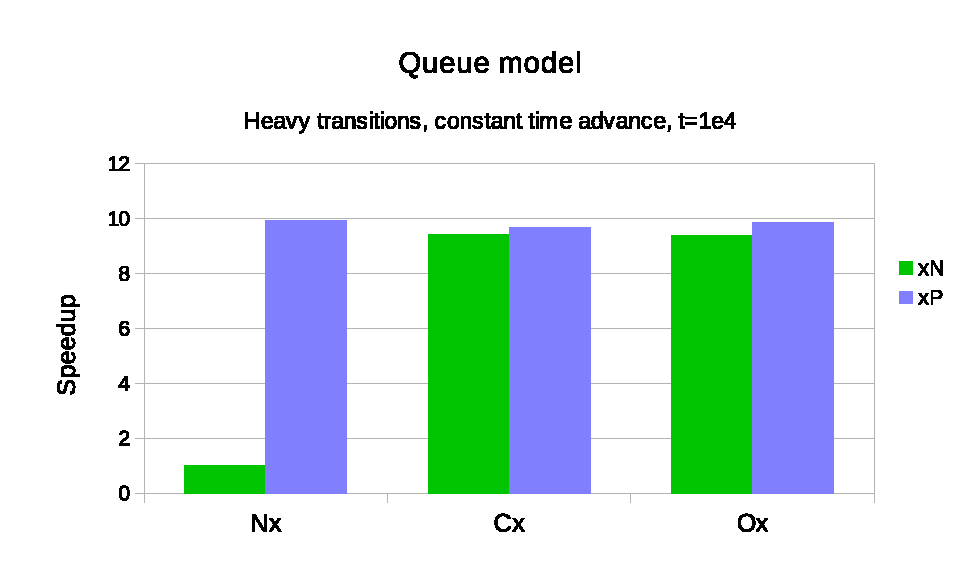
\includegraphics[width=\columnwidth]{fig/pdevs_fixed_sleep.eps}
	\caption{Queue speedup benchmark for PDEVS and synchronization with maximal concurrent events and significant computational load}
	\label{fig:pdevs_plot_fixed_sleep}
\end{figure}

\begin{figure}
	\center
	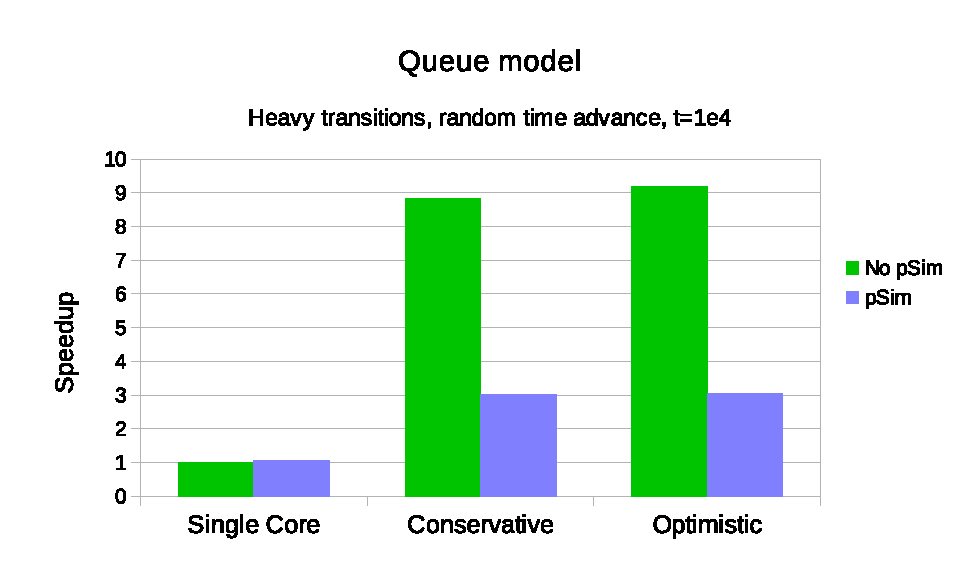
\includegraphics[width=\columnwidth]{fig/pdevs_random_sleep.eps}
	\caption{Queue speedup benchmark for PDEVS and synchronization with randomized events and significant computational load}
	\label{fig:pdevs_plot_random_sleep}
\end{figure}

\begin{figure}
	\center
	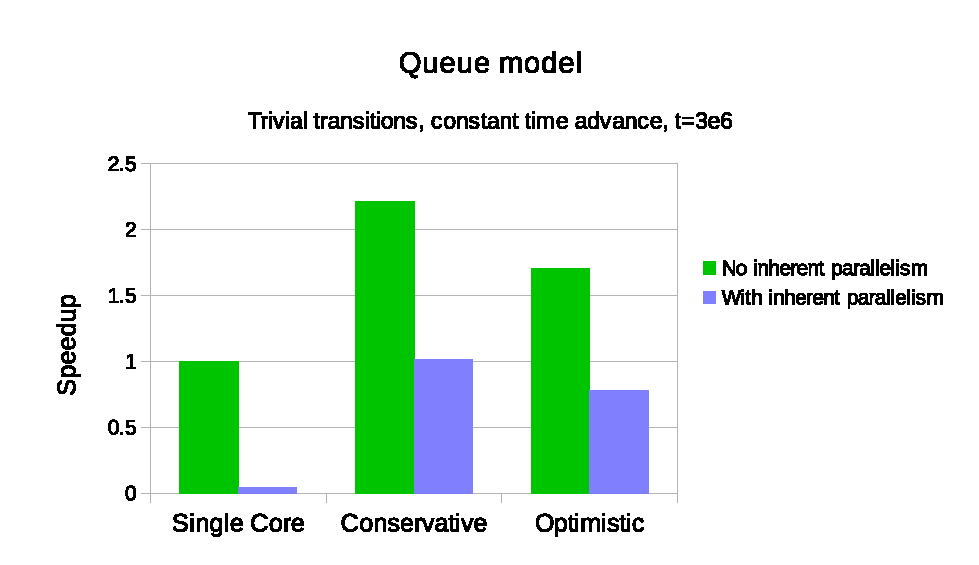
\includegraphics[width=\columnwidth]{fig/pdevs_no_sleep.eps}
	\caption{Queue speedup benchmark for PDEVS and synchronization with maximal concurrent events and trivial computational load}
	\label{fig:pdevs_plot_no_sleep}
\end{figure} 